\begin{multicols}{3}
\byline{Интервю с учителя по физическо възпитание и спорт  – Вели Аслан}{Слави и Христо, ХД}

От колко време сте учител в ГПНЕ „Гьоте”?

Три години и половина.

И как се чувствате в гимназията?

Чувствам се много добре, работя с прекрасни деца.  Единственото нещо, което не ми харесва в тази обстановка  е,  че родителите са прекалено взискателни към моя предмет и това донякъде спъва и спира работата ми с децата.

А как се отнасят учениците към предмета ви?

Те нямат много голям избор и се отнасят с уважение и влизат в часовете подготвени, както се изисква от тях, така че към учениците нямам никаква забележка по отношение на карането на часовете.

Има ли нещо,  което искате да промените в гимназията и в учениците?

О, да..Определено има  много неща, които искам да променя и в учениците,  и в гимназията и  полека си правя моите стъпки в тази посока. В гимназията бих променил базата, начина по който  се подават нещата. Като цяло съм склонен да направя големи промени , но за съжаление нямам тази власт и възможност да го направя, затова се старая до колкото ми позволява предмета и изобщо сферата в която съм учител да направя децата по –добри, да ги променям от гледна точка на това  да бъдат по-добри като хора, като личности.

Ще ни разкажете ли нещо повече за себе си? С какво се занимавате и като учител по ФВС,  водите ли здравословен начин на живот?

Занимавам се с бойни изкуства и това само по себе си говори,  че начинът ми на живот е не само здравословен, но и от душевна гледна точка е на доста високо ниво, поради простата причина,  че бойните изкуства изискват такъв тип живот  и начин на мислене. Освен с бойни изкуства се занимавам и с много други неща, социално-обществена личност съм, старая се да помагам на колкото се може повече хора, за мен това е основна мисия.Парите не са ми самоцел и за мен е по-важно да оставя едно вътрешно удоволетворение  в себе си затова,  че съм постигнал  или съм успял да променя нещо към по-добро, отколкото да ставам сутринта и да се чудя как да изкарам определени пари,  за да мога да си покрия някакви нужди. Съвета ми към всички е да постъпват по този начин, защото когато парите не са ти самоцел- те си идват така или иначе сами по себе си. Много  е важно човек да се  грижи за себе си и това е едно от нещата на които се стремя да науча моите ученици – да се грижат добре за себе си, за да могат след това да дават  пример и на другите.

Какви са целите Ви? Мечтаете ли за нещо?

Имам много цели в живота си...Човек трябва да има цел и да я преследва.Може да звучи  странно, но моята цел е колкото се може повече да се издигна от духовна гледна точка , да усъвършенствам себе си  до такава степен , че живота ми да стане изключително щастлив и приятен. За мен една от важните цели е да разпространя това с което се занимавам- Традиционно Джу Джицу, то да достигне до повече хора, защото това е нещо много  стойностно  и качествено като занимание и дава много положителни аспекти като самочувствие, самоувереност , желание да помагаш. Отделно чрез него се придобиват  много сериозни умения  и  една от важните  ми мисии е да разпространя това бойно изкуство  доколкото се може до повече хора , а в личен план нещата, които искам да постигна  са по-скоро душевен мир и спокойствие,  това е най-важното нещо за мен.

Има ли нещо , което искате да кажете на читателите, някакво послание?

смихвайте се повече, правете добри неща за хората около вас и вярвайте в себе си! 
\end{multicols}
% \noindent \begin{window}[2,r, 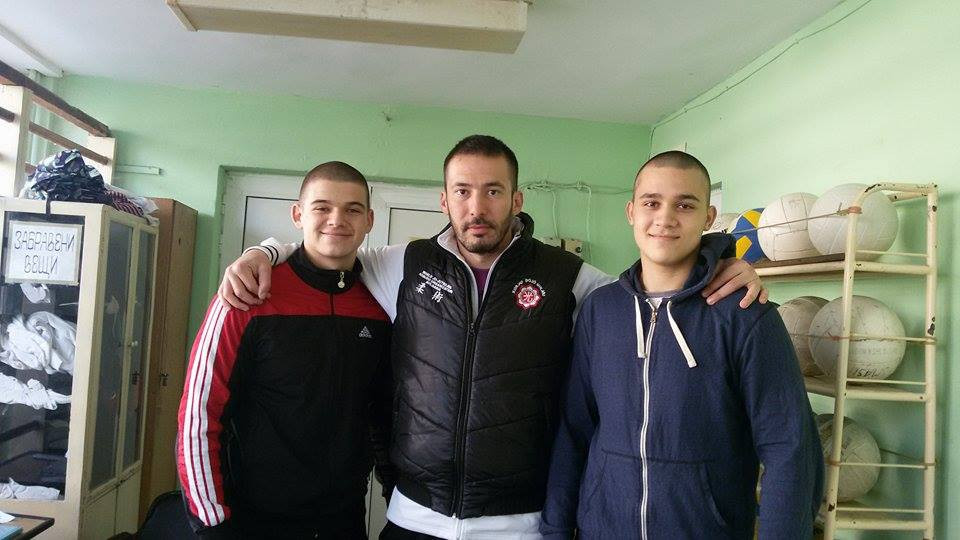
\includegraphics[width=5.1in]{./Aslan/Aslan.jpg},] \end{window}

\begin{center}
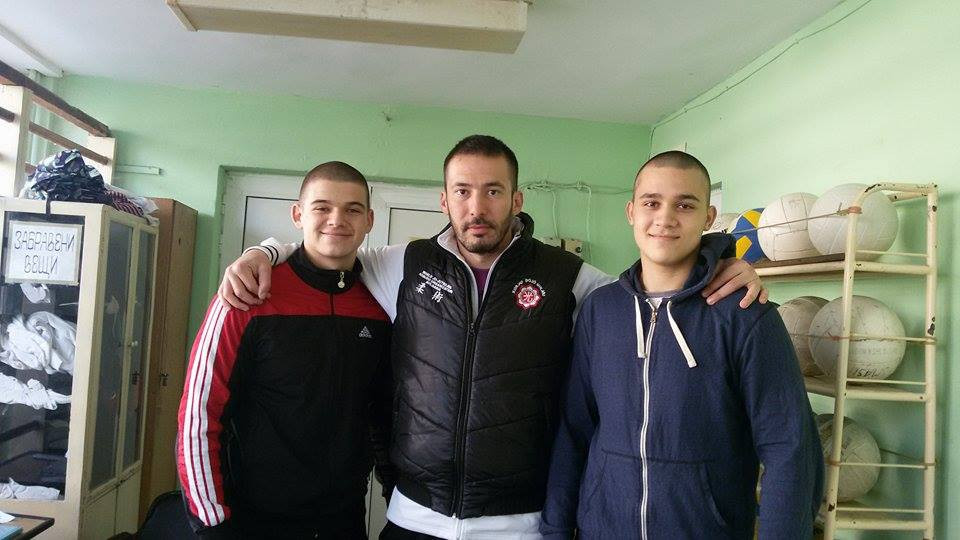
\includegraphics[width=5.7in]{./Aslan/Aslan.jpg}
\end{center}

 
\closearticle


